\documentclass[10pt]{examdesign}
\usepackage{amsmath}
\usepackage{enumitem}
\usepackage{amsfonts}
\usepackage{pgfplots}
\usepackage{pifont}
\usepackage{graphicx}
\usepackage{fancyhdr}
\usepackage{cancel}
\usepackage[american]{circuitikz}

\SectionFont{\large\sffamily}
\Fullpages
\ContinuousNumbering
\usepackage{ulem}
\ProportionalBlanks{2}


\DefineAnswerWrapper{}{}
\NumberOfVersions{3}
%\IncludeFromFile{foobar.tex}
\examname{\Large{9 Weeks Exam}}
\class {\Large Physics}

\def \namedata {Name: \hrulefill\\ 
	Date: \hrulefill \\
	Period: \hrulefill \\
	Primary Peer Reviewer: \hrulefill 
	\\
			\begin{tabular}{| p{1cm} | p{1cm} | p{1 cm} | p{1cm} |}
	\hline
		+1 & 0 & -1 & $\Sigma$ 
		\\
		\hline
		& & & \vspace{.5cm}
		\\ \hline
	
	\end{tabular}
	\\
 \vspace{-.6in}
	
}




\begin{document}




\begin{multiplechoice} [title={Multiple Choice},
	rearrange=yes]
\textit{Choose the best answer to each question.}

	
	
	
	
	\begin{question}
Which of the following measurements is the closest to 1x10\textsuperscript{-2} m? 
	\choice{The diameter of an atom}
	\choice[!]{The width of a student's finger}
	\choice{The height of a school teacher}
	\choice{The length of a football field}

	\end{question}


\begin{question}
A train is traveling to the right with a constant speed $v_t$.  Two identical spheres are rolling on the floor of one train car.  In the frame of reference of the train, the spheres are moving directly toward each other with a speed $v_p$, parallel to the train's motion, as shown in the figure above.  A person is standing outside the train as it passes by.  What are the velocities that the person would measure of each of the spheres as the train passes by? 

\begin{center}
		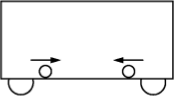
\includegraphics[height=0.5in]{train2.png}  
\end{center}



\choice{Left Sphere: $v_p + v_t$ \hspace{0.25in} Right sphere: $v_p + v_t$}
\choice{Left Sphere: $v_p - v_t$ \hspace{0.25in} Right sphere: $v_p + v_t$}
\choice[!]{Left Sphere: $v_p + v_t$ \hspace{0.25in} Right sphere: $v_p - v_t$}
\choice{Left Sphere: $v_p - v_t$ \hspace{0.25in} Right sphere: $v_p - v_t$}

\end{question}

\begin{block}
 \textit{	The following two questions refer to the following information:}
 	
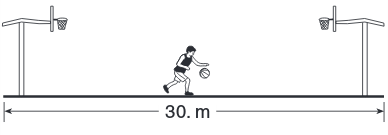
\includegraphics[height=0.5in]{bball.png} 

During a drill in basketball practice, a player runs the length of a 30 meter court and back.  The player does this three times in 60 seconds. 

\begin{question}
	What is the magnitude of the player's displacement at the end of the drill? (Hint: Magnitude means number only and not direction.)
	\choice[!]{0 m}
	\choice{30 m}
	\choice{60 m}
	\choice{180 m}
\end{question}


	\begin{question}
What is the player's average speed during this drill? 
	\choice {0 m/s}
	\choice {0.5 m/s}
	\choice[!]{3 m/s}
	\choice {30 m/s}
\end{question}
\end{block}


	\begin{question}
An airplane starts from rest and accelerates at a constant rate along a runway for a distance d in time t.  If the same airplane were to accelerate at the same rate, what would be the time it takes the airplane to go a distance 2d, in terms of t?
	\choice {$\frac{t}{2}$}
	\choice[!] {$\sqrt{2}t$}
	\choice {2t}
	\choice {4t}
\end{question}

\begin{question}
A student standing on the roof of a 50-meter tall buliding kicks a stone with an initial horizontal speed of 4 m/s, as shown in the diagram.  How much time is required for the stone to reach the ground below? 
\choice[!]{3.19 s}
\choice{5.10 s}
\choice{10.2 s}
\choice{12.5 s}

\vspace{-1in} \hspace{2 in} 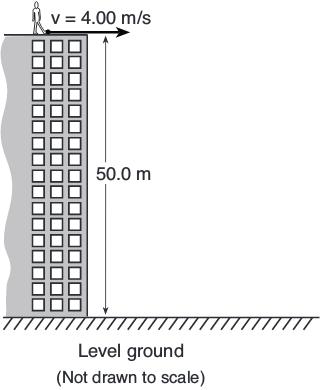
\includegraphics[height=1in]{building.png}

	\end{question}

\begin{question}
During the 2012 Olympics in London, Usain Bolt ran 100 meters in 9.63 seconds.  What was his average speed? 
\choice{0.096 m/s}
\choice{4.557 m/s}
\choice[!]{10.384 m/s}
\choice{968 m/s}

	
\end{question}


\begin{question}
Diana is in a bowling tournament when she rolls a bowling ball with an initial speed of 12 m/s toward the pins.  Due to friction, the bowling ball decelerates at a rate of 0.3 m/s\textsuperscript{2}.  What is the final speed of the bowling ball when it hits the pins, 18.9 meters away?
\choice{0.812 m/s}
\choice[!]{11.518 m/s}
\choice{12.464 m/s}
\choice{132.66 m/s}

\end{question}


\begin{question}
A blue car and a red car are racing.  Both cars start from a stop and accelerate, each at a different constant rate.  The blue car crosses the finish line in 10 seconds, and the red car crosses the finish line in 20 seconds.  Compared to the blue car's final velocity, the red car's final velocity was - 
\choice{$\frac{1}{4}$  the blue car's final velocity}
\choice[!]{$\frac{1}{2}$ the blue car's final velocity}
\choice{the same as the blue car's final velocity}
\choice{2 times the blue car's final velocity}
	\end{question}

\begin{question}
	
A lion is running at a constant speed toward a gazelle that is standing still, as shown in the top figure.  After several seconds, the gazelle notices the lion and accelerates directly toward him, hoping to pass the lion and force him to reverse direction.  As the gazelle accelerates toward and past the lion, the lion changes direction and accelerates in pursuit of the gazelle.   The lion and Gazelle eventually reach constant but different speeds. 

\begin{center} 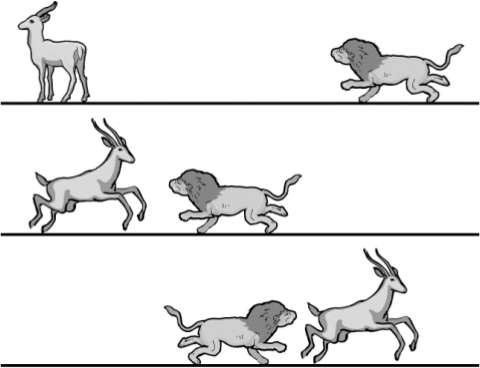
\includegraphics[height=0.75in]{lg1.png} \end{center}


 Which of the following sets of graphs shows a reasonable representation of the velocities of the lion and the gazelle as functions of time? 
 
	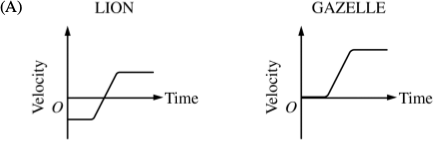
\includegraphics[height=0.75in]{lga.png} \hspace{1in} 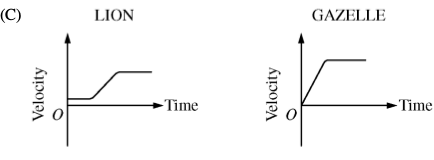
\includegraphics[height=0.75in]{lgc.png} \\	
	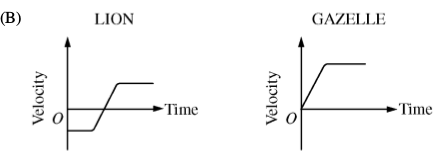
\includegraphics[height=0.75in]{lgb.png} \hspace{1in} 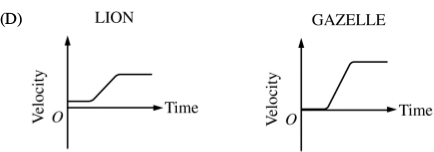
\includegraphics[height=0.75in]{lgd.png}

\end{question}

\begin{question}
An airplane is traveling north at 220 m/s when it encounters a 50 m/s crosswind from west to east.  What is the resultant speed of the plane, rounded to the nearest whole number? 
\choice{170 m/s}
\choice{214 m/s}
\choice[!]{226 m/s}
\choice{270 m/s}
	\end{question}




\begin{question}
Gravity on the moon is approximately 1/6th that of gravity on the earth.  An astronaut on the moon drops  a rock from a height, h, that causes it to hit the surface of the moon 1 second later. If a rock were dropped from the same height on earth, how long does it take to hit the ground?
\choice{$\frac{1}{6}$ s}
\choice[!]{$\sqrt{\frac{1}{6}}$ s}
\choice{$\frac{1}{36}$ s}
\choice{1 s}
	\end{question}

\begin{question}
	During a baseball game, a player hits a ball directly up.  It is in the air for a total of 6.2 seconds.  At the top of its path, the acceleration of the ball is - 
\choice{0 m/s\textsuperscript{2}}
\choice[!]{9.81 m/s\textsuperscript{2} downward}
\choice{30.411 m/s\textsuperscript{2} upward}
\choice{50.227 m/s\textsuperscript{2} upward}
\end{question}

\begin{block}
The following information applies to the next two questions:




\begin{question}
		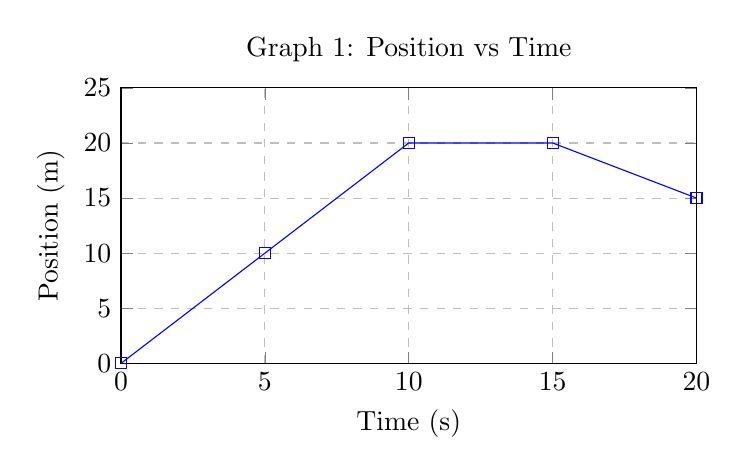
\begin{tikzpicture}
	\begin{axis}[
	title={Graph 1: Position vs Time},
	xlabel={Time (s)},
	ylabel={Position (m)},
	xmin=0, xmax=20,
	ymin=0, ymax=25,
	xtick={0,5,10,15,20},
	ytick={0,5,10,15,20,25},
	ymajorgrids=true,
	xmajorgrids=true,
	grid style=dashed,
	legend pos=south east,
	height=2in,
	width=3.5in
	]
	
	\addplot[
	color=blue,
	mark=square,
	]
	coordinates {
		(0,0)(5,10)(10,20)(15,20)(20,15)};
	
	
	
	
	
	\end{axis}
	\end{tikzpicture}

What is the average speed of this object from 0 to 10 seconds?
\choice{100 m/s}
\choice{20 m/s}
\choice[!]{2 m/s}
\choice{0.5 m/s}
\end{question}

\begin{question}
During what time interval is the object traveling backward?
\choice{0-10 seconds}
\choice{10-15 seconds}
\choice[!]{15-20 seconds}
\choice{The object does not travel backwards at any time.}

	\end{question}

\end{block}

	\begin{question}
	A man rolls a ball up a hill with an initial speed of 2 m/s. 10 seconds later, it is traveling at 5.2 m/s down the hill.  What is the ball's acceleration?
	\choice [!]{-0.72 m/s\textsuperscript{2}}
	\choice {0.32 m/s\textsuperscript{2}}
	\choice {52 m/s\textsuperscript{2}}
	\choice {10791.859 m/s\textsuperscript{2}}
\end{question}

\begin{question}
	What is the best description of acceleration?
\choice {How fast an object is traveling.}
\choice {How far an object travels in a certain amount of time.}
\choice {How much an object slides or spins.}
\choice [!]{Speeding up, slowing down, or changing direction.}
\end{question}

\begin{question}
	Which of the following numbers is greatest?
	\choice{$2 \times 10^{-7}$}
	\choice[!]{$3 \times 10^6$}
	\choice{$4 \times 10^{5} $}
	\choice{$5 \times 10^{4} $}
	
\end{question}


\begin{question}
A person walks 5.0 kilometers north, then 5.0 kilometers east. Which of the following is closest to the person's net displacement?
\choice{10 km Northeast}
\choice{7.1 km Northwest}
\choice[!]{7.1 km Northeast}
\choice{10 km Northwest}
\end{question}

\begin{question}

The graph below represents the relationship between the distance traveled and time elapsed for an object in motion.  

		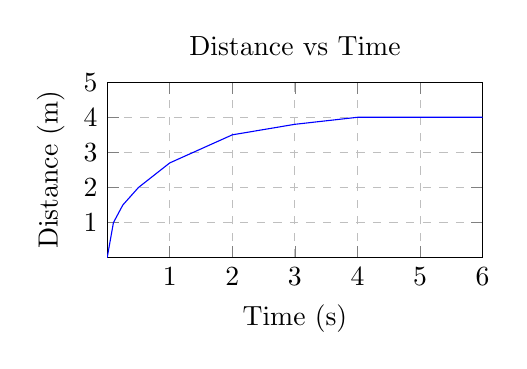
\begin{tikzpicture}
\begin{axis}[
title={Distance vs Time},
xlabel={Time (s)},
ylabel={Distance (m)},
xmin=0, xmax=6,
ymin=0, ymax=5,
xtick={1,2,3,4,5,6},
ytick={1,2,3,4,5},
ymajorgrids=true,
xmajorgrids=true,
grid style=dashed,
legend pos=south east,
height=1.5in,
width=2.5in
]

\addplot[
color=blue,
]
coordinates {
	(0,0)(.1,1)(.25,1.5)(.5,2)(1,2.7)(2,3.5)(3,3.8)(4,4)(5,4)(6,4)};
\end{axis}
\end{tikzpicture}

What is the instantaneous speed of the object 5.0 seconds after the start?

\choice[!]{0 m/s}
\choice{2 m/s}
\choice{4 m/s}
\choice{5 m/s}

	\end{question}

\begin{question}
A car is traveling eastward along a straight road. The graph below represents the velocity of the car as a function of time, t.

		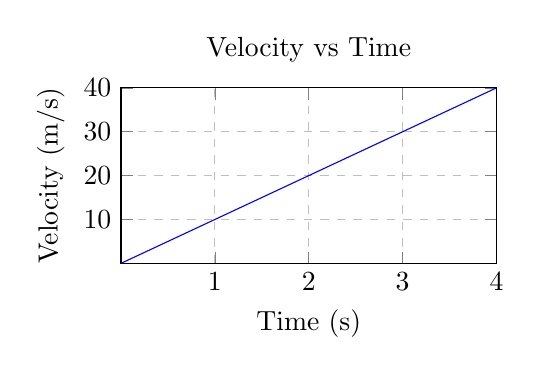
\begin{tikzpicture}
\begin{axis}[
title={Velocity vs Time},
xlabel={Time (s)},
ylabel={Velocity (m/s)},
xmin=0, xmax=4,
ymin=0, ymax=40,
xtick={1,2,3,4},
ytick={10,20,30,40},
ymajorgrids=true,
xmajorgrids=true,
grid style=dashed,
legend pos=south east,
height=1.5in,
width=2.5in
]

\addplot[
color=blue,
]
coordinates {
	(0,0)(1,10)(2,20)(3,30)(4,40)};
\end{axis}
\end{tikzpicture}

What is the magnitude of the displacement of the car from t = 2.0 seconds to t = 4.0 seconds?
\choice{20. m}
\choice{40. m}
\choice[!]{60. m}
\choice{80. m}
	\end{question}



\begin{question}
	The speed-time graph shown below represents the motion of an object:
	
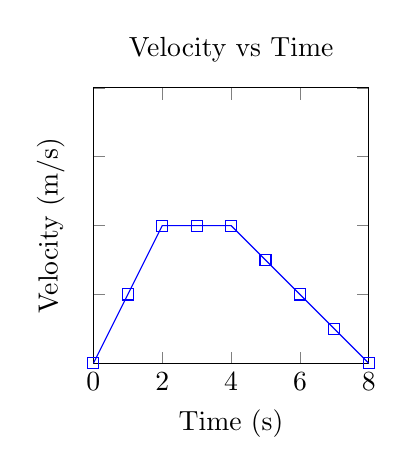
\begin{tikzpicture}
\pgfplotsset{compat=1.5.1}
\begin{axis}[
title={Velocity vs Time},
xlabel={Time (s)},
ylabel={Velocity (m/s)},
xmin=0, xmax=8,
ymin=0, ymax=8,
yticklabels={,,}
ymajorgrids=false,
xmajorgrids=false,
grid style=dashed,
legend pos=south east,
height=2in,
width=2in
]
\addplot[
color=blue,
mark=square,
]
coordinates {
	(0,0)(1,2)(2,4)(3,4)(4,4)(5,3)(6,2)(7,1)(8,0)
};
\end{axis}
\end{tikzpicture}

What is the best description for the motion of the object from 4 to 8 seconds?
\choice[!]{The object is moving forward as it slows down and stops.}
\choice{The object is moving backward at a constant speed.}
\choice{The object is moving forward at a constant speed.}
\choice{The object is not moving.}

\end{question}

\begin{question}
	The following graph shows the relationship between the force on an object and the acceleration of an object.:
	
	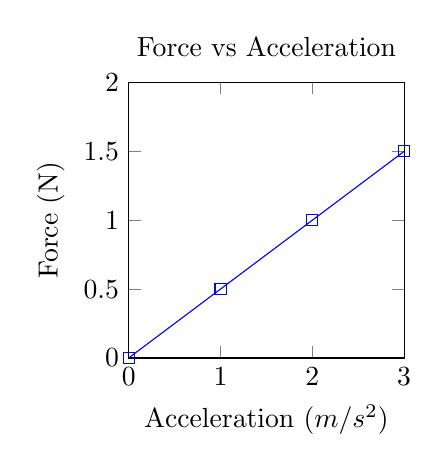
\begin{tikzpicture}
	\pgfplotsset{compat=1.5.1}
	\begin{axis}[
	title={Force vs Acceleration},
	xlabel={Acceleration ($m/s^2$)},
	ylabel={Force (N)},
	xmin=0, xmax=3,
	ymin=0, ymax=2,
	ymajorgrids=false,
	xmajorgrids=false,
	grid style=dashed,
	legend pos=south east,
	height=2in,
	width=2in
	]
	\addplot[
	color=blue,
	mark=square,
	]
	coordinates {
		(0,0)(1,.5)(2,1)(3,1.5)
	};
	\end{axis}
	\end{tikzpicture}
	
	What is the Mass of the object?
	\choice[!]{0.5 kg}
	\choice{1 kg}
	\choice{2 kg}
	\choice{2.25 kg}
	
\end{question}


\begin{question}
When a projectile is launched horizontally, the \textbf{time} the projectile is in the air depends on - 
\choice{The initial speed only}
\choice[!]{The initial height only}
\choice{Both the initial height and the initial speed}
\choice{Neither initial height nor initial speed}
\end{question}


\begin{question}
When a projectile is launched horizontally, the \textbf{range} of the projectile depends on - 
\choice{The initial speed only}
\choice{The initial height only}
\choice[!]{Both the initial height and the initial speed}
\choice{Neither initial height nor initial speed}
\end{question}





\begin{question}
An object with an initial speed of 4.0 m/s accelerates uniformly at 2.0 m/s\textsuperscript{2} in the direction of its motion for a distance of 5.0 meters. What is the
final speed of the object? 
\choice[!]{6.0 m/s}
\choice{10. m/s}
\choice{14 m/s}
\choice{36 m/s}
	\end{question}

\begin{question}
A student drops an object from the top of a building 19.6 meters from the ground. How long does it take the object to fall to the ground? 
\choice[!]{2 seconds}
\choice{3 seconds}
\choice{4 seconds}
\choice{19.6 seconds}
\end{question}

\begin{question}
A bus is moving forward at 20 m/s.  A student on the bus throws a tennis ball horizontally at 15 m/s toward the front of the bus.  From the perspective of an observer standing on the sidewalk outside the bus, the tennis ball appears to move at - 
	\choice{5 m/s}
	\choice{15 m/s}
	\choice{20 m/s}
	\choice[!]{35 m/s}
	\end{question}

\begin{question}
	A car accelerates at $2 m/s^2$.  What is its final velocity?
	\choice{0 m/s}
	\choice{2 m/s}
	\choice{4 m/s}
	\choice[!]{There is not enough information to solve this problem.}
\end{question}

\begin{block}
The next two questions refer to the following information:

	A ball is thrown directly upward with an initial speed of 12 m/s. 
	
\begin{question}
  How high does the ball go?
	\choice{1.223 m}
	\choice{4.35 m}
	\choice[!]{7.339 m}
	\choice{117.72 m}
\end{question}

\begin{question}
What is the velocity of the ball when it reaches the top of its trajectory?
\choice[!]{0 m/s}
\choice{9.81 m/s downward}
\choice{12 m/s upward}
\choice{There is not enough information to determine the answer to this question.}

	\end{question}



\end{block}

\begin{question}
A blue sphere and a red sphere with the same diameter are released from rest at the top of a ramp. The red sphere takes a longer time to reach the bottom of the ramp. The spheres are then rolled off a horizontal table at the same time with the same speed and fall freely to the floor. Which sphere reaches the floor first? 
\choice{The red sphere}
\choice{The blue sphere}
\choice{The sphere with the greater mass}
\choice[!]{Neither; the spheres reach the floor at the same time.}
\end{question}

\begin{question}
	An astronaut is standing on the surface of the moon.  (The Moon has no atmosphere, and $g_{moon} = 8.87 m/s^2$)  He holds a hammer in one hand and a feather in the other hand, the same distance from the surface.  He drops both at the same time.  Which is the best description of what happens?
	\choice{The feather lands first.}
	\choice{The hammer lands first.}
	\choice[!]{Both objects land at the same time.}
	\choice{Both objects float away.}
\end{question}




\end{multiplechoice}

\pagebreak
\begin{multiplechoice} [title={Multiple Correct Multiple Choice},
	rearrange=yes]
	\textit{For the following question, \textbf{choose two} correct answers.  No credit will be given for incorrect or partially correct answers.  Mark \textbf{both} answers clearly.} 



\begin{question}
Barney is running to the east at 5 m/s.  Gwenda is 30 meters away from Barney and running toward him at 7 m/s, but we do not know if she is east of him or west of him. Which of the following times could it take Gwenda to meet Barney? (CHOOSE TWO)
	\choice[!]{15 s}
	\choice{13 s}
	\choice{6 s}
	\choice{4.286 s}
	\choice[!]{2.5 s}
\end{question}

\begin{question}
A car starts from rest and accelerates at a constant rate of 3 m/s\textsuperscript{2}.  What additional information could be used to calculate the final velocity of the car? (CHOOSE TWO)
\choice[!]{The time the car is accelerating.}
\choice[!]{The total displacement of the car.}
\choice{The direction that the car is traveling in.}
\choice{The horizontal and vertical components of the car's velocity.}

\end{question}

\begin{question}
Which of the following quantities are scalars? (CHOOSE TWO)
\choice[!]{Distance}
\choice{Displacement}
\choice[!]{Speed}
\choice{Velocity}
\choice{Acceleration}
\end{question}

\begin{question}
Which of the following objects are accelerating? (CHOOSE TWO)
\choice[!]{A train that slows down as it pulls into the station.}
\choice{A car that is stopped at a red light.}
\choice{A boat traveling at a constant speed on calm water.}
\choice[!]{A racecar that is going around a turn at a constant speed.}
\choice{An airplane traveling in a straight line at a constant speed.}
	\end{question}


\begin{question}
A woman throws a rock horizontally off of a cliff.  Which of the following statements are true concerning the time it takes for the rock to hit the ground.  (CHOOSE TWO)
\choice{The harder the rock is thrown, the longer the rock will take to reach the ground.}
\choice{The harder the rock is thrown, the less time the rock will take to reach the ground.}
\choice[!]{The speed that the rock is thrown horizontally has no effect on the time it takes the rock to reach the ground.}
\choice[!]{The time it takes the rock to reach the ground is the same as the time it would take a rock to reach the ground when dropped from the same height.}
\choice{A rock that is thrown horizontally will always reach the ground faster than a rock that is dropped from the same height.}

	\end{question}




\end{multiplechoice}

\end{document}



